% Context budget — compact variant for cheat-sheet column.
% Narrower bar width (6cm vs 10cm in tutorial), shorter labels.
% Same color palette + threshold annotations.
\documentclass[tikz,border=4mm]{standalone}
\usepackage{tikz}
\usetikzlibrary{positioning, calc}

\begin{document}
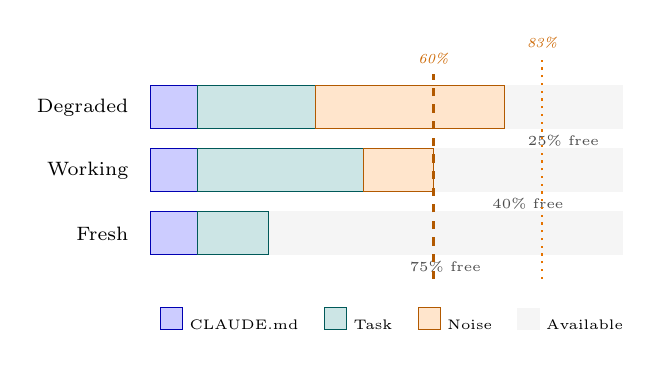
\begin{tikzpicture}[
  font=\sffamily,
  bar/.style={
    minimum height=0.55cm, anchor=south west,
    font=\tiny\bfseries, align=center
  },
  lbl/.style={font=\scriptsize, anchor=east},
  pct/.style={font=\tiny, text=gray!60!black},
  thresh60/.style={dashed, thick, draw=orange!70!black},
  thresh83/.style={dotted, thick, draw=orange!90!black},
  threshlbl/.style={font=\tiny\itshape, text=orange!80!black},
]
  \def\barwidth{6cm}

  % --- Fresh session ---
  \node[lbl] at (-0.15, 0.27) {Fresh};
  \node[bar, fill=blue!20, draw=blue!70!black, minimum width=0.10*\barwidth] at (0, 0) {};
  \node[bar, fill=teal!20, draw=teal!70!black, minimum width=0.15*\barwidth] at (0.10*\barwidth, 0) {};
  \node[bar, fill=gray!8, minimum width=0.75*\barwidth] at (0.25*\barwidth, 0) {};
  \node[pct] at (0.625*\barwidth, -0.15) {75\% free};

  % --- Working session ---
  \node[lbl] at (-0.15, 1.07) {Working};
  \node[bar, fill=blue!20, draw=blue!70!black, minimum width=0.10*\barwidth] at (0, 0.8) {};
  \node[bar, fill=teal!20, draw=teal!70!black, minimum width=0.35*\barwidth] at (0.10*\barwidth, 0.8) {};
  \node[bar, fill=orange!20, draw=orange!70!black, minimum width=0.15*\barwidth] at (0.45*\barwidth, 0.8) {};
  \node[bar, fill=gray!8, minimum width=0.40*\barwidth] at (0.60*\barwidth, 0.8) {};
  \node[pct] at (0.80*\barwidth, 0.65) {40\% free};

  % --- Degraded session ---
  \node[lbl] at (-0.15, 1.87) {Degraded};
  \node[bar, fill=blue!20, draw=blue!70!black, minimum width=0.10*\barwidth] at (0, 1.6) {};
  \node[bar, fill=teal!20, draw=teal!70!black, minimum width=0.25*\barwidth] at (0.10*\barwidth, 1.6) {};
  \node[bar, fill=orange!20, draw=orange!70!black, minimum width=0.40*\barwidth] at (0.35*\barwidth, 1.6) {};
  \node[bar, fill=gray!8, minimum width=0.25*\barwidth] at (0.75*\barwidth, 1.6) {};
  \node[pct] at (0.875*\barwidth, 1.45) {25\% free};

  % --- Threshold annotations ---
  \draw[thresh60] (0.60*\barwidth, -0.3) -- (0.60*\barwidth, 2.3)
    node[above, threshlbl] {60\%};
  \draw[thresh83] (0.83*\barwidth, -0.3) -- (0.83*\barwidth, 2.5)
    node[above, threshlbl] {83\%};

  % Legend (replaces in-bar labels which were too cramped at compact size)
  \node[font=\tiny, anchor=west] at (0, -0.8) {%
    \tikz{\node[fill=blue!20, draw=blue!70!black, minimum width=8pt, minimum height=8pt] {};} CLAUDE.md \quad%
    \tikz{\node[fill=teal!20, draw=teal!70!black, minimum width=8pt, minimum height=8pt] {};} Task \quad%
    \tikz{\node[fill=orange!20, draw=orange!70!black, minimum width=8pt, minimum height=8pt] {};} Noise \quad%
    \tikz{\node[fill=gray!8, minimum width=8pt, minimum height=8pt] {};} Available%
  };

\end{tikzpicture}
\end{document}
